\documentclass[aspectratio=169,11pt,t]{beamer}

% ============================================================
% Theme and typography
% ============================================================

\usetheme{Madrid}
\usecolortheme{default}
\usefonttheme{professionalfonts}

\setbeamertemplate{navigation symbols}{}
\setbeamertemplate{headline}{}

\setbeamertemplate{footline}{%
  \leavevmode\hbox{%
  \begin{beamercolorbox}[wd=.82\paperwidth,ht=2.5ex,dp=1.0ex,leftskip=.8em]{author in head/foot}
    CSCI 6461 --- Computer Systems Architecture
  \end{beamercolorbox}%
  \begin{beamercolorbox}[wd=.18\paperwidth,ht=2.5ex,dp=1.0ex,rightskip=.8em]{date in head/foot}
    \hfill\insertframenumber/\inserttotalframenumber
  \end{beamercolorbox}}
}

\setbeamersize{text margin left=0.65cm,text margin right=0.65cm}

\setbeamerfont{frametitle}{size=\Large, series=\bfseries}
\setbeamerfont{block title}{size=\normalsize, series=\bfseries}
\setbeamertemplate{blocks}[rounded][shadow=false]

\addtobeamertemplate{block begin}{\vspace{0.1em}}{\vspace{0.1em}}
\addtobeamertemplate{block end}{}{\vspace{0.2em}}

\setbeamertemplate{itemize/enumerate body begin}{\setlength{\itemsep}{4pt}}
\setbeamertemplate{itemize/enumerate subbody begin}{\setlength{\itemsep}{2pt}}

% ============================================================
% Packages
% ============================================================

\usepackage[T1]{fontenc}
\usepackage{lmodern}
\usepackage{iftex}
\ifPDFTeX
  \usepackage[scale=0.92]{sourcecodepro}
\else
  \usepackage{fontspec}
  \setmonofont{Source Code Pro}[Scale=0.92]
\fi
\usepackage{amsmath}
\usepackage{booktabs}
\usepackage{array}
\usepackage{colortbl}
\usepackage{tikz}
\usepackage{adjustbox}

\usetikzlibrary{arrows.meta,positioning,shapes.geometric,calc,decorations.pathreplacing}

% ============================================================
% Colors
% ============================================================

\definecolor{navy}{RGB}{24,43,68}
\definecolor{deepblue}{RGB}{45,88,130}
\definecolor{lightblue}{RGB}{235,242,250}
\definecolor{softgray}{RGB}{245,247,250}
\definecolor{darkgray}{RGB}{25,28,32}
\definecolor{gold}{RGB}{200,145,35}
\definecolor{softgreen}{RGB}{226,242,232}
\definecolor{softorange}{RGB}{253,238,215}
\definecolor{softpurple}{RGB}{238,234,250}

\setbeamercolor{palette primary}{bg=navy,fg=white}
\setbeamercolor{palette secondary}{bg=deepblue,fg=white}
\setbeamercolor{frametitle}{bg=navy,fg=white}
\setbeamercolor{title}{fg=white}
\setbeamercolor{subtitle}{fg=white}
\setbeamercolor{author}{fg=white}
\setbeamercolor{date}{fg=white}
\setbeamercolor{titlelike}{fg=white}
\setbeamercolor{block title}{bg=deepblue,fg=white}
\setbeamercolor{block body}{bg=lightblue,fg=darkgray}
\setbeamercolor{normal text}{fg=darkgray,bg=white}

% ============================================================
% Formatting shortcuts
% ============================================================

\setlength{\parskip}{0pt}
\newcommand{\key}[1]{\textbf{#1}}
\newcommand{\bits}[1]{\texttt{#1}}
\newcommand{\hex}[1]{\texttt{0x#1}}
\newcommand{\code}[1]{\texttt{#1}}

\newcommand{\bfld}[5]{%
  \pgfmathsetmacro{\cx}{#1 + #3/2}%
  \fill[#5] (#1,#2) rectangle ++(#3,0.72);%
  \draw[navy,line width=0.7pt] (#1,#2) rectangle ++(#3,0.72);%
  \node[font=\scriptsize,align=center,text=darkgray] at (\cx,#2+0.36) {#4};%
}

\newcommand{\sectiondivider}[2]{%
\begin{frame}[plain]
\begin{tikzpicture}[remember picture,overlay]
\fill[navy] (current page.south west) rectangle (current page.north east);
\fill[gold] (current page.south west) rectangle ([yshift=.15cm]current page.south east);
\end{tikzpicture}
\vspace*{\fill}
\begin{minipage}{0.94\textwidth}
\raggedright
\hyphenpenalty=10000
\exhyphenpenalty=10000
{\color{gold}\large\bfseries #1\par}
\vspace{0.3cm}
{\color{white}\fontsize{22}{26}\selectfont\bfseries #2\par}
\end{minipage}
\vspace*{\fill}
\end{frame}
}

\tikzset{
  unit/.style={draw=navy,line width=0.8pt,rounded corners=2pt,fill=lightblue,minimum width=2.35cm,minimum height=0.82cm,align=center,font=\small},
  state/.style={unit,fill=gold!24},
  logic/.style={unit,fill=softgreen},
  mux/.style={trapezium, trapezium left angle=70, trapezium right angle=110, draw=navy, line width=0.8pt, fill=softorange, minimum width=0.62cm, minimum height=0.95cm, font=\scriptsize, align=center},
  arr/.style={-{Stealth[length=2.2mm]},draw=navy,line width=0.8pt},
  bus/.style={-{Stealth[length=2.2mm]},draw=navy,line width=1.0pt},
  ctrl/.style={-{Stealth[length=2.0mm]},draw=deepblue,line width=0.8pt,dashed}
}
\tikzset{
  memblock/.style={state,minimum width=3.15cm,minimum height=1.05cm},
  regblock/.style={state,minimum width=2.35cm,minimum height=1.45cm}
}


% Reusable register-file symbol based on the ARM datapath convention.
\newcommand{\RegFileSymbol}[1][0.42]{%
\begin{tikzpicture}[
    scale=#1,
    transform shape,
    font=\sffamily\color{black!55},
    thick_line/.style={draw=black!55, ultra thick},
    pin_line/.style={draw=black!55, very thick}
]
    \draw[thick_line] (0,0) rectangle (3.6,4.6);

    \draw[thick_line] (0.3,4.6) -- (0.6,4.3) -- (0.9,4.6);

    \draw[pin_line] (0.6,4.6) -- (0.6,4.9)
      node[above,inner sep=3pt,font=\sffamily\large\color{black!55}] {CLK};

    \draw[pin_line] (1.8,4.6) -- (1.8,4.9);
    \node[below,font=\sffamily\large\color{black!55}] at (1.8,4.6) {WE3};

    \draw[pin_line] (-0.6,3.9) -- (0,3.9);
    \node[right,font=\sffamily\large\color{black!55}] at (0.1,3.9) {A1};

    \draw[pin_line] (-0.6,2.6) -- (0,2.6);
    \node[right,font=\sffamily\large\color{black!55}] at (0.1,2.6) {A2};

    \draw[pin_line] (-0.6,1.6) -- (0,1.6);
    \node[right,font=\sffamily\large\color{black!55}] at (0.1,1.6) {A3};

    \draw[pin_line] (-0.6,0.9) -- (0,0.9);
    \node[right,font=\sffamily\large\color{black!55}] at (0.1,0.9) {WD3};

    \draw[pin_line] (-0.6,0.3) -- (0,0.3);
    \node[right,font=\sffamily\large\color{black!55}] at (0.1,0.3) {PC};

    \draw[pin_line] (3.6,3.9) -- (4.2,3.9);
    \node[left,font=\sffamily\large\color{black!55}] at (3.5,3.9) {RD1};

    \draw[pin_line] (3.6,2.6) -- (4.2,2.6);
    \node[left,font=\sffamily\large\color{black!55}] at (3.5,2.6) {RD2};

    \node[align=center,font=\sffamily\Large\bfseries\color{black!55}]
      at (2.1,1.3) {Register\\[-0.5ex]File};
\end{tikzpicture}%
}


% Reusable instruction-memory symbol.
\newcommand{\InstrMemSymbol}[1][0.42]{%
\begin{tikzpicture}[
    scale=#1,
    transform shape,
    font=\sffamily\color{black!55},
    thick_line/.style={draw=black!55, ultra thick},
    pin_line/.style={draw=black!55, very thick}
]
    % Main Instruction Memory Box
    \draw[thick_line] (0,0) rectangle (3.2,4.2);

    % Left Input
    \draw[pin_line] (-0.6,2.8) -- (0,2.8);
    \node[right,font=\sffamily\large\color{black!55}] at (0.2,2.8) {A};

    % Right Output
    \draw[pin_line] (3.2,2.8) -- (4.0,2.8);
    \node[left,font=\sffamily\large\color{black!55}] at (3.0,2.8) {RD};

    % Vertical Bus Line
    \draw[thick_line] (4.0,0.0) -- (4.0,5.0);

    % External Instr label (vertical)
    \node[align=left,font=\sffamily\large\color{black!55},rotate=-90] at (3.6,3.6) {Instr};

    % Inner Label
    \node[align=center,font=\sffamily\Large\bfseries\color{black!55}] at (1.6,1.4) {Instruction\\[-0.5ex]Memory};
\end{tikzpicture}%
}




% Reusable data-memory symbol.
\newcommand{\DataMemSymbol}[1][0.42]{%
\begin{tikzpicture}[
    scale=#1,
    transform shape,
    font=\sffamily\color{black!55},
    thick_line/.style={draw=black!55, ultra thick},
    pin_line/.style={draw=black!55, very thick}
]
    \draw[thick_line] (0,0) rectangle (3.0,5.0);

    \draw[thick_line] (0.3,5.0) -- (0.6,4.7) -- (0.9,5.0);

    \draw[pin_line] (0.6,5.0) -- (0.6,5.3)
      node[above,font=\sffamily\large\color{black!55}] {CLK};
    \node[below,font=\sffamily\large\color{black!55}] at (1.8,5.0) {WE};

    \draw[pin_line] (-0.6,3.6) -- (0,3.6);
    \node[right,font=\sffamily\large\color{black!55}] at (0.1,3.6) {A};

    \draw[pin_line] (-0.6,0.4) -- (0,0.4);
    \node[right,font=\sffamily\large\color{black!55}] at (0.1,0.4) {WD};

    \draw[pin_line] (3.0,3.6) -- (3.6,3.6);
    \node[left,font=\sffamily\large\color{black!55}] at (2.9,3.6) {RD};

    \node[align=center,font=\sffamily\Large\bfseries\color{black!55}]
      at (1.5,2.2) {Data\\[-0.5ex]Memory};
\end{tikzpicture}%
}



% Reusable ALU symbol.
\newcommand{\ALUSymbol}[1][0.34]{%
\begin{tikzpicture}[
    scale=#1,
    transform shape,
    font=\sffamily\color{black!55},
    thick_line/.style={draw=black!55, ultra thick},
    pin_line/.style={draw=black!55, very thick}
]
    \draw[thick_line]
        (0, 3.0) --
        (2.0, 2.6) --
        (2.0, -0.6) --
        (0, -1.0) --
        (0, 0.6) --
        (1.0, 1.0) --
        (0, 1.4) --
        cycle;

    \draw[pin_line] (-1.8, 2.2) -- (0, 2.2);
    \node[above,font=\sffamily\large\color{black!55},inner sep=2pt] at (-0.9, 2.2) {SrcA};

    \draw[pin_line] (-1.8, -0.2) -- (0, -0.2);
    \node[above,font=\sffamily\large\color{black!55},inner sep=2pt] at (-0.9, -0.2) {SrcB};

    \draw[pin_line] (2.0, 1.0) -- (2.6, 1.0);

    \draw[pin_line] (1.0, 3.5) -- (1.0, 2.8);

    \node[rotate=90,font=\sffamily\Large\color{black!55}] at (1.4, 1.0) {ALU};
\end{tikzpicture}%
}


% Reusable immediate-extension symbol.
\newcommand{\ExtendSymbol}[1][0.42]{%
\begin{tikzpicture}[
    scale=#1,
    transform shape,
    font=\sffamily\color{black!55},
    thick_line/.style={draw=black!55, ultra thick},
    pin_line/.style={draw=black!55, very thick}
]
    \draw[thick_line]
        (0, 0) --
        (4.0, 0) --
        (4.0, 1.2) --
        (0, 0.5) --
        cycle;

    \draw[pin_line] (-0.6, 0.25) -- (0, 0.25);
    \draw[pin_line] (4.0, 0.6) -- (4.6, 0.6);

    \node[align=center,font=\sffamily\Large\bfseries\color{black!55}] at (2.0, 0.45) {Extend};
\end{tikzpicture}%
}

% ============================================================

\tikzset{
  stage/.style={draw=navy,fill=lightblue,rounded corners=2pt,minimum width=2.1cm,minimum height=1.05cm,align=center,font=\small},
  preg/.style={draw=navy,fill=gold!28,minimum width=0.18cm,minimum height=1.65cm,inner sep=0pt},
  flow/.style={-{Stealth[length=2mm]},draw=navy,line width=0.9pt},
  bypass/.style={-{Stealth[length=2mm]},draw=gold!85!black,line width=1.2pt},
  kill/.style={draw=red!65!black,fill=red!10,rounded corners=2pt,align=center,font=\small},
  tcell/.style={draw=white,line width=1pt,minimum width=0.76cm,minimum height=0.54cm,inner sep=1pt,font=\footnotesize\ttfamily}
}
\title[Topic 9]{Pipelining Fundamentals \& the 5-Stage RISC Pipeline}
\subtitle{AArch64 instruction flow, pipeline state, hazards, and performance}
\author{Computer Systems Architecture}
\date{}
\begin{document}
\begin{frame}[plain]
\begin{tikzpicture}[remember picture,overlay]
\fill[navy] (current page.south west) rectangle (current page.north east);
\fill[gold] (current page.south west) rectangle ([yshift=.15cm]current page.south east);
\end{tikzpicture}
\vspace*{\fill}
\begin{minipage}{0.94\textwidth}
{\color{gold}\normalsize\bfseries CSCI 6461 \;|\; TOPIC 9\par}
\vspace{0.3cm}
{\color{white}\fontsize{24}{28}\selectfont\bfseries Pipelining Fundamentals\\[0.12cm]\& the 5-Stage RISC Pipeline\par}
\vspace{0.35cm}
{\color{white!80}\large AArch64 instruction flow, pipeline state,\\hazards, and performance\par}
\end{minipage}
\vfill
{\color{white!70}\small Dr. J. Burns\par}
\vspace*{\fill}
\end{frame}

\sectiondivider{PART 1}{Pipelining Principles and Timing}

\begin{frame}{The AArch64 Teaching Model}

\begin{itemize}\setlength{\itemsep}{5pt}
  \item \key{ISA behavior:} execute real A64 instructions while preserving their register, memory, and control-flow effects.
  \item \key{Implementation:} a single-issue, in-order pipeline with stages IF, ID, EX, MEM, and WB.
  \item \key{Timing assumptions:} one cycle per stage, separate instruction/data access, cache hits, and branch resolution in EX.
  \item \key{Register timing:} a WB write is visible to an ID read in the same cycle.
  \item \key{Scope:} simple integer ALU operations, offset \code{ldr}/\code{str}, and \code{b}/\code{cbz}/\code{cbnz}. Use \code{x0}--\code{x30} in the worked examples.
\end{itemize}
\vspace{0.05cm}
\begin{block}{ISA and Microarchitecture}
The AArch64 ISA does not prescribe five stages. The diagrams describe the teaching implementation used in this lecture.
\end{block}

\end{frame}

\begin{frame}{Overlapping Instructions}

\begin{center}
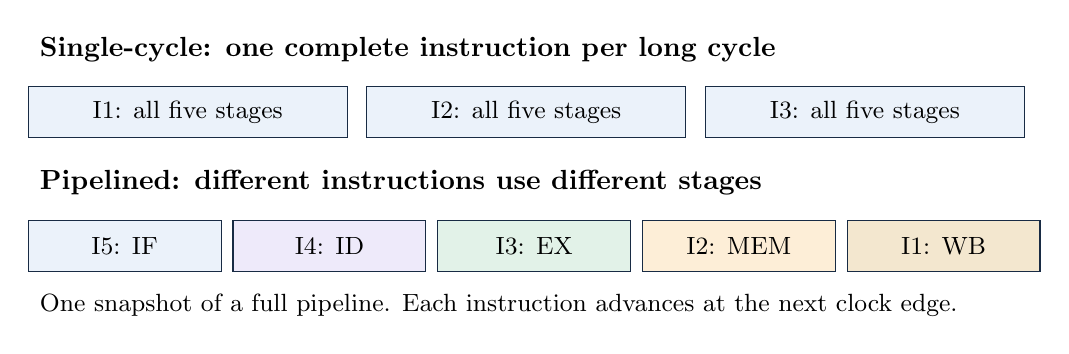
\begin{tikzpicture}[x=1cm,y=1cm,font=\small]
\node[anchor=west,font=\bfseries] at (0,2.6) {Single-cycle: one complete instruction per long cycle};
\foreach \x/\lab in {0/I1,4.3/I2,8.6/I3} {
  \node[draw=navy,fill=lightblue,minimum width=4.05cm,minimum height=.65cm] at (\x+2,1.8) {\lab: all five stages};
}
\node[anchor=west,font=\bfseries] at (0,.9) {Pipelined: different instructions use different stages};
\foreach \x/\lab/\col in {0/I5: IF/lightblue,2.6/I4: ID/softpurple,5.2/I3: EX/softgreen,7.8/I2: MEM/softorange,10.4/I1: WB/gold!22} {
  \node[draw=navy,fill=\col,minimum width=2.45cm,minimum height=.65cm] at (\x+1.2,0.1) {\lab};
}
\node[anchor=west] at (0,-.65) {One snapshot of a full pipeline. Each instruction advances at the next clock edge.};
\end{tikzpicture}
\end{center}

\begin{itemize}\setlength{\itemsep}{7pt}
  \item The hardware overlaps work on several instructions without changing program order.
  \item The shorter clock permits more instructions to finish per unit of time once the pipeline is full.
\end{itemize}

\end{frame}

\begin{frame}{Clock Period and Stage Balance}
\begin{center}
\small
\renewcommand{\arraystretch}{1.28}
\setlength{\tabcolsep}{5pt}
\rowcolors{2}{softgray}{white}
\begin{tabular}{llllll}
\toprule
\rowcolor{white}
\textbf{Stage} & \textbf{IF} & \textbf{ID} & \textbf{EX} & \textbf{MEM} & \textbf{WB} \\
\midrule
Delay (picoseconds, ps) & 200 & 100 & 200 & 200 & 100 \\
\bottomrule
\end{tabular}
\end{center}

\small One picosecond is $10^{-12}$ seconds. Assume 20 ps of register and clocking overhead.\normalsize
\begin{block}{Illustrative Timing Calculation}
Single-cycle period: $T_{\mathrm{single}} = \sum t_{\mathrm{stage}}+t_{\mathrm{reg}} = 800+20=820$ ps.\\[0.12cm]
Pipeline period: $T_{\mathrm{pipe}} = \max(t_{\mathrm{stage}}) + t_{\mathrm{reg}} = 200+20 = 220$ ps.
\end{block}

\begin{itemize}\setlength{\itemsep}{6pt}
  \item The slowest stage limits the clock. Spare time in ID and WB does not shorten a 200 ps stage.
  \item For a long independent stream, the ideal speedup approaches $820/220 \approx 3.73$.
\end{itemize}

\end{frame}

\begin{frame}{Reading a Pipeline Timing Diagram}
\begin{center}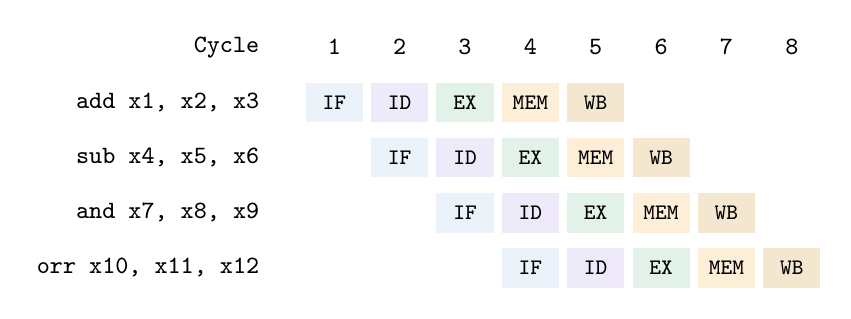
\begin{tikzpicture}[x=0.83cm,y=0.70cm]
\node[anchor=east,font=\small\ttfamily\bfseries] at (0,0) {Cycle};
\node[font=\small\ttfamily] at (1,0) {1};
\node[font=\small\ttfamily] at (2,0) {2};
\node[font=\small\ttfamily] at (3,0) {3};
\node[font=\small\ttfamily] at (4,0) {4};
\node[font=\small\ttfamily] at (5,0) {5};
\node[font=\small\ttfamily] at (6,0) {6};
\node[font=\small\ttfamily] at (7,0) {7};
\node[font=\small\ttfamily] at (8,0) {8};
\node[anchor=east,font=\small\ttfamily,align=right] at (0,-1) {\code{add x1, x2, x3}};
\node[tcell,fill=lightblue] (r1c1) at (1,-1) {IF};
\node[tcell,fill=softpurple] (r1c2) at (2,-1) {ID};
\node[tcell,fill=softgreen] (r1c3) at (3,-1) {EX};
\node[tcell,fill=softorange] (r1c4) at (4,-1) {MEM};
\node[tcell,fill=gold!22] (r1c5) at (5,-1) {WB};
\node[anchor=east,font=\small\ttfamily,align=right] at (0,-2) {\code{sub x4, x5, x6}};
\node[tcell,fill=lightblue] (r2c2) at (2,-2) {IF};
\node[tcell,fill=softpurple] (r2c3) at (3,-2) {ID};
\node[tcell,fill=softgreen] (r2c4) at (4,-2) {EX};
\node[tcell,fill=softorange] (r2c5) at (5,-2) {MEM};
\node[tcell,fill=gold!22] (r2c6) at (6,-2) {WB};
\node[anchor=east,font=\small\ttfamily,align=right] at (0,-3) {\code{and x7, x8, x9}};
\node[tcell,fill=lightblue] (r3c3) at (3,-3) {IF};
\node[tcell,fill=softpurple] (r3c4) at (4,-3) {ID};
\node[tcell,fill=softgreen] (r3c5) at (5,-3) {EX};
\node[tcell,fill=softorange] (r3c6) at (6,-3) {MEM};
\node[tcell,fill=gold!22] (r3c7) at (7,-3) {WB};
\node[anchor=east,font=\small\ttfamily,align=right] at (0,-4) {\code{orr x10, x11, x12}};
\node[tcell,fill=lightblue] (r4c4) at (4,-4) {IF};
\node[tcell,fill=softpurple] (r4c5) at (5,-4) {ID};
\node[tcell,fill=softgreen] (r4c6) at (6,-4) {EX};
\node[tcell,fill=softorange] (r4c7) at (7,-4) {MEM};
\node[tcell,fill=gold!22] (r4c8) at (8,-4) {WB};


\end{tikzpicture}\end{center}
\begin{itemize}\setlength{\itemsep}{7pt}
  \item Read a row to follow one instruction. Read a column to see the work occurring in one cycle.
  \item Four independent instructions take $4+4=8$ cycles from first fetch to final WB.
  \item The initial fill and final drain prevent a short sequence from achieving one instruction per cycle overall.
\end{itemize}

\end{frame}

\begin{frame}{Latency, Throughput, and Ideal CPI}
\begin{center}
\small
\renewcommand{\arraystretch}{1.28}
\setlength{\tabcolsep}{5pt}
\rowcolors{2}{softgray}{white}
\begin{tabular}{>{\raggedright\arraybackslash}p{3.8cm}>{\raggedright\arraybackslash}p{9.2cm}}
\toprule
\rowcolor{white}
\textbf{Quantity} & \textbf{Meaning in this model} \\
\midrule
Instruction latency & Five cycles from IF through WB: $5\times220=1100$ ps. \\
Steady-state throughput & One instruction reaches WB every 220 ps when there are no hazards. \\
Finite sequence & $N$ instructions require $N+4$ cycles in an initially empty pipeline. \\
Cycles per instruction (CPI) & $\mathrm{CPI}=(N+4)/N$ without stalls or flushes. \\
\bottomrule
\end{tabular}
\end{center}
\vspace{0.1cm}
\begin{block}{Pipelining Improves Throughput}
The example pipeline has a longer per-instruction latency than the 820 ps single-cycle design, but finishes a long instruction stream sooner.
\end{block}

\end{frame}

\sectiondivider{PART 2}{The Five Stages and Pipeline State}

\begin{frame}{The 5-Stage Datapath}

\begin{center}
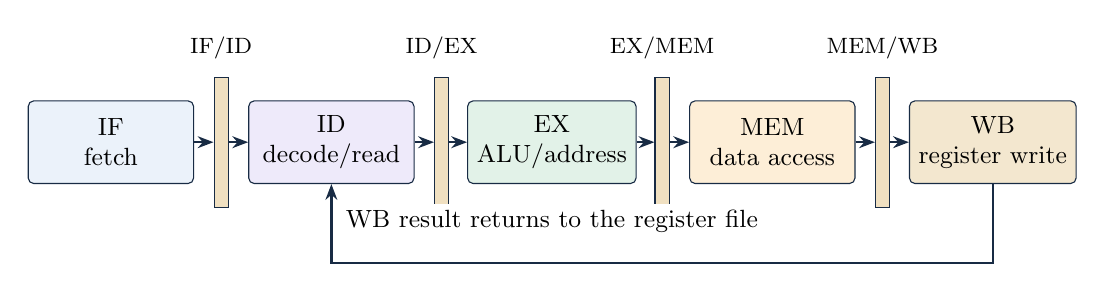
\begin{tikzpicture}[font=\small]
\node[stage] (f) at (0,0) {IF\\fetch};
\node[stage,fill=softpurple] (d) at (2.8,0) {ID\\decode/read};
\node[stage,fill=softgreen] (e) at (5.6,0) {EX\\ALU/address};
\node[stage,fill=softorange] (m) at (8.4,0) {MEM\\data access};
\node[stage,fill=gold!22] (w) at (11.2,0) {WB\\register write};
\foreach \x/\lab/\name in {1.4/{IF/ID}/a,4.2/{ID/EX}/b,7.0/{EX/MEM}/c,9.8/{MEM/WB}/d} {
 \node[preg] (p\name) at (\x,0) {};
 \node[font=\footnotesize,above=.1cm] at (p\name.north) {\lab};
}
\draw[flow] (f)--(pa);\draw[flow] (pa)--(d);
\draw[flow] (d)--(pb);\draw[flow] (pb)--(e);
\draw[flow] (e)--(pc);\draw[flow] (pc)--(m);
\draw[flow] (m)--(pd);\draw[flow] (pd)--(w);
\draw[flow] (w.south) -- ++(0,-1) -| (d.south);
\node[font=\small,fill=white,inner sep=2pt] at (5.6,-1) {WB result returns to the register file};
\end{tikzpicture}
\end{center}

\begin{itemize}\setlength{\itemsep}{7pt}
  \item Pipeline registers hold each stage\textquotesingle s outputs until the next clock edge.
  \item Different instructions occupy these stages concurrently.
  \item An instruction passes through every stage, but only enables the actions it needs.
\end{itemize}

\end{frame}

\begin{frame}{IF and ID: Fetch, Decode, and Read}

\begin{columns}[T,onlytextwidth]
\column{.48\textwidth}
\begin{block}{IF: Instruction Fetch}
\begin{itemize}\setlength{\itemsep}{6pt}
\item Use the PC to fetch one 32-bit A64 instruction.
\item Select $PC+4$ for the next sequential instruction.
\item Keep the instruction\textquotesingle s own PC in IF/ID for later PC-relative calculations.
\end{itemize}
\end{block}
\column{.48\textwidth}
\begin{block}{ID: Decode and Register Read}
\begin{itemize}\setlength{\itemsep}{6pt}
\item Identify the instruction\textquotesingle s source and destination registers.
\item Read operands and generate an immediate value.
\item Produce control signals and record them in ID/EX.
\end{itemize}
\end{block}
\end{columns}
\vspace{.25cm}
\code{ldr x7, [x5, \#16]}: read \code{x5}, record destination \code{x7}, and generate the byte offset 16.
\note{ISA reference: Arm, A64 ISA and Compilers, fixed 32-bit instructions.}

\end{frame}

\begin{frame}{EX: Arithmetic, Addresses, and Branches}
\begin{center}
\small
\renewcommand{\arraystretch}{1.28}
\setlength{\tabcolsep}{5pt}
\rowcolors{2}{softgray}{white}
\begin{tabular}{>{\raggedright\arraybackslash}p{5.6cm}>{\raggedright\arraybackslash}p{7.4cm}}
\toprule
\rowcolor{white}
\textbf{Instruction} & \textbf{EX-stage operation} \\
\midrule
\code{add x7, x5, x6} & Add the two operand values; result is destined for \code{x7}. \\
\code{ldr x7, [x5, \#16]} & Compute effective address $x5+16$. \\
\code{str x7, [x5, \#16]} & Compute effective address $x5+16$; preserve store data separately. \\
\code{cbz x7, .Lzero} & Test the operand for zero and calculate the target from the branch\textquotesingle s PC. \\
\bottomrule
\end{tabular}
\end{center}
\begin{block}{Values Needed in EX}
The forwarding network can replace an old ID operand with a newer result. Store data and the \code{cbz}/\code{cbnz} test operand also use this network in our model.
\end{block}

\end{frame}

\begin{frame}{MEM and WB: Memory Effects and Register Results}

\begin{columns}[T,onlytextwidth]
\column{.48\textwidth}
\begin{block}{MEM: Data Memory Access}
\begin{itemize}\setlength{\itemsep}{6pt}
\item \code{ldr}: read memory at the effective address.
\item \code{str}: write the saved store-data value to memory.
\item ALU instructions and branches pass through without data-memory access.
\end{itemize}
\end{block}
\column{.48\textwidth}
\begin{block}{WB: Register Writeback}
\begin{itemize}\setlength{\itemsep}{6pt}
\item Select the ALU result or loaded memory value.
\item Write the saved destination register if \code{RegWrite = 1}.
\item \code{str} and the branches used here have \code{RegWrite = 0}.
\end{itemize}
\end{block}
\end{columns}
\vspace{.25cm}
An ALU result is available at the end of EX. A loaded value becomes available at the end of MEM.

\end{frame}

\begin{frame}{Pipeline Registers Carry Data and Control}
\begin{center}
\small
\renewcommand{\arraystretch}{1.28}
\setlength{\tabcolsep}{5pt}
\rowcolors{2}{softgray}{white}
\begin{tabular}{>{\raggedright\arraybackslash}p{3.0cm}>{\raggedright\arraybackslash}p{10.0cm}}
\toprule
\rowcolor{white}
\textbf{Boundary} & \textbf{Information retained for the same instruction} \\
\midrule
IF/ID & Instruction word, instruction PC, valid bit. \\
ID/EX & Operand values, source/destination register numbers, immediate, PC, EX/MEM/WB controls. \\
EX/MEM & ALU result or address, corrected store data, destination number, MEM/WB controls. \\
MEM/WB & Loaded data, ALU result, destination number, WB controls. \\
\bottomrule
\end{tabular}
\end{center}

\begin{itemize}\setlength{\itemsep}{5pt}
  \item For \code{ldr x7, [x5, \#16]}, destination number 7 must travel all the way to WB.
  \item WB cannot use the destination field of the newer instruction currently in ID.
  \item A valid bit or disabled write controls allows an empty slot to move safely through the pipeline.
\end{itemize}

\end{frame}

\begin{frame}{Worked Load and Store: The Same Address Path}

\small\key{Assume:} \code{x5 = 0x1000}, memory at \code{0x1010} holds 42, and \code{x7 = 99} initially.
\begin{center}
\small
\renewcommand{\arraystretch}{1.28}
\setlength{\tabcolsep}{5pt}
\rowcolors{2}{softgray}{white}
\begin{tabular}{>{\raggedright\arraybackslash}p{1.5cm}>{\raggedright\arraybackslash}p{5.7cm}>{\raggedright\arraybackslash}p{5.7cm}}
\toprule
\rowcolor{white}
\textbf{Stage} & \textbf{\code{ldr x7, [x5, \#16]}} & \textbf{\code{str x7, [x5, \#16]}} \\
\midrule
IF & Fetch the instruction. & Fetch the instruction. \\
ID & Read \code{x5}; save destination 7. & Read \code{x5} and store source \code{x7}. \\
EX & Address $=\hex{1010}$. & Address $=\hex{1010}$; store data $=99$. \\
MEM & Read the 64-bit value 42. & Write the 64-bit value 99. \\
WB & Write 42 into \code{x7}. & No register write. \\
\bottomrule
\end{tabular}
\end{center}

\normalsize
Treat the two examples independently. The unsigned-offset encoding has \code{imm12 = 2}, giving $2\times8=16$ bytes; \code{x5} is unchanged.
\note{Arm A64 LDR (immediate), unsigned offset: encoded imm12 scales by access size. STR has the corresponding unsigned-offset form.}

\end{frame}

\sectiondivider{PART 3}{Hazards, Forwarding, and Stalls}

\begin{frame}{Three Classes of Pipeline Hazard}
\begin{center}
\small
\renewcommand{\arraystretch}{1.28}
\setlength{\tabcolsep}{5pt}
\rowcolors{2}{softgray}{white}
\begin{tabular}{>{\raggedright\arraybackslash}p{2.2cm}>{\raggedright\arraybackslash}p{6.3cm}>{\raggedright\arraybackslash}p{4.2cm}}
\toprule
\rowcolor{white}
\textbf{Hazard} & \textbf{What prevents normal progress?} & \textbf{Example} \\
\midrule
Structural & Two stages need the same hardware resource at once. & IF and MEM compete for one memory port. \\
Data & A consumer needs a result that an older instruction has not yet supplied. & \code{add} produces the operand of a following \code{sub}. \\
Control & The correct next PC is not yet known. & \code{cbz} may redirect instruction fetch. \\
\bottomrule
\end{tabular}
\end{center}

\begin{center}
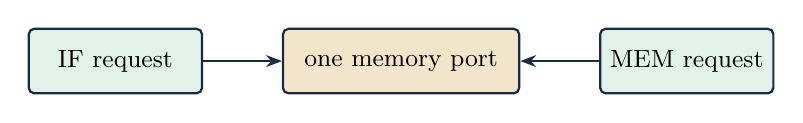
\begin{tikzpicture}[font=\small,node distance=1.0cm]
\node[logic,minimum width=2.2cm] (f) {IF request};
\node[state,right=of f,minimum width=3.0cm] (mem) {one memory port};
\node[logic,right=of mem,minimum width=2.2cm] (m) {MEM request};
\draw[flow] (f)--(mem);\draw[flow] (m)--(mem);
\end{tikzpicture}
\end{center}
Our model avoids this structural conflict with separate instruction and data access.

\end{frame}

\begin{frame}{RAW Dependence: Waiting for a Register Result}
\begin{block}{A read-after-write (RAW) dependence}
\ttfamily\small
\begin{tabular}{@{}l@{}}
add x7, x5, x6 \\
sub x8, x7, x9
\end{tabular}
\end{block}
\begin{center}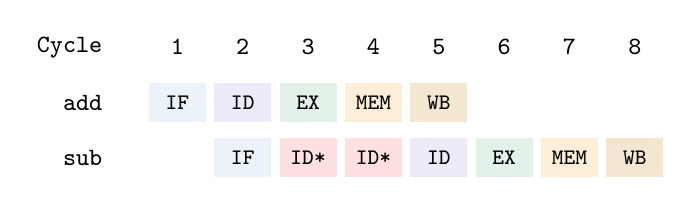
\begin{tikzpicture}[x=0.83cm,y=0.70cm]
\node[anchor=east,font=\small\ttfamily\bfseries] at (0,0) {Cycle};
\node[font=\small\ttfamily] at (1,0) {1};
\node[font=\small\ttfamily] at (2,0) {2};
\node[font=\small\ttfamily] at (3,0) {3};
\node[font=\small\ttfamily] at (4,0) {4};
\node[font=\small\ttfamily] at (5,0) {5};
\node[font=\small\ttfamily] at (6,0) {6};
\node[font=\small\ttfamily] at (7,0) {7};
\node[font=\small\ttfamily] at (8,0) {8};
\node[anchor=east,font=\small\ttfamily,align=right] at (0,-1) {\code{add}};
\node[tcell,fill=lightblue] (r1c1) at (1,-1) {IF};
\node[tcell,fill=softpurple] (r1c2) at (2,-1) {ID};
\node[tcell,fill=softgreen] (r1c3) at (3,-1) {EX};
\node[tcell,fill=softorange] (r1c4) at (4,-1) {MEM};
\node[tcell,fill=gold!22] (r1c5) at (5,-1) {WB};
\node[anchor=east,font=\small\ttfamily,align=right] at (0,-2) {\code{sub}};
\node[tcell,fill=lightblue] (r2c2) at (2,-2) {IF};
\node[tcell,fill=red!12] (r2c3) at (3,-2) {ID*};
\node[tcell,fill=red!12] (r2c4) at (4,-2) {ID*};
\node[tcell,fill=softpurple] (r2c5) at (5,-2) {ID};
\node[tcell,fill=softgreen] (r2c6) at (6,-2) {EX};
\node[tcell,fill=softorange] (r2c7) at (7,-2) {MEM};
\node[tcell,fill=gold!22] (r2c8) at (8,-2) {WB};


\end{tikzpicture}\end{center}
\begin{itemize}\setlength{\itemsep}{5pt}
  \item Without forwarding, \code{sub} must wait for \code{add} to write \code{x7}.
  \item WB writes before ID reads in cycle 5, so the consumer reaches EX in cycle 6: two stall cycles.
  \item \code{ID*} marks an instruction held in ID. The dependency is on a value, not just adjacent instructions.
\end{itemize}

\end{frame}

\begin{frame}{Forwarding an ALU Result}

\code{add x7, x5, x6} \qquad followed by \qquad \code{sub x8, x7, x9}
\begin{center}
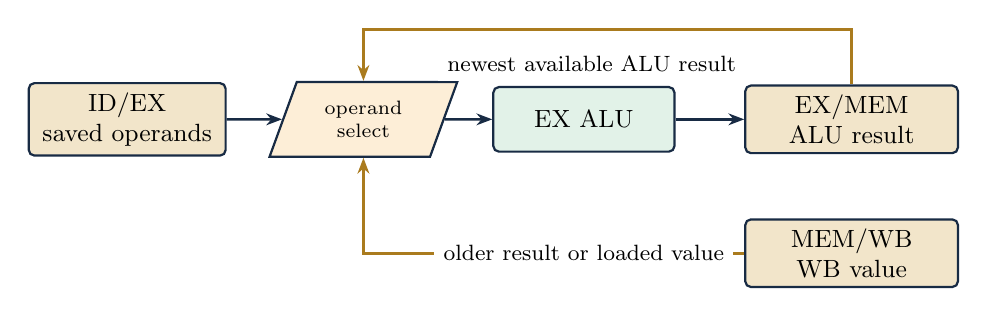
\begin{tikzpicture}[font=\small]
\node[state,minimum width=2.5cm] (id) at (0,0) {ID/EX\\saved operands};
\node[mux] (mux) at (3,0) {operand\\select};
\node[logic,minimum width=2.3cm] (alu) at (5.8,0) {EX ALU};
\node[state,minimum width=2.7cm] (em) at (9.2,0) {EX/MEM\\ALU result};
\node[state,minimum width=2.7cm] (mw) at (9.2,-1.7) {MEM/WB\\WB value};
\draw[flow] (id)--(mux);\draw[flow] (mux)--(alu);\draw[flow] (alu)--(em);
\draw[bypass] (em.north)--++(0,.7)-| (mux.north);
\node[font=\footnotesize,fill=white] at (5.9,.7) {newest available ALU result};
\draw[bypass] (mw.west)-| (mux.south);
\node[font=\footnotesize,fill=white] at (5.8,-1.7) {older result or loaded value};
\end{tikzpicture}
\end{center}

\begin{itemize}\setlength{\itemsep}{5pt}
  \item \code{add} finishes EX in cycle 3. EX/MEM supplies its result to \code{sub} in EX in cycle 4: no stall.
  \item Match valid register writes to source operands. If two results match, select the newest one.
  \item Never forward a load\textquotesingle s address as loaded data.
\end{itemize}

\end{frame}

\begin{frame}{The Load-Use Hazard: One Cycle Too Soon}
\begin{block}{An immediate consumer of a loaded value}
\ttfamily\small
\begin{tabular}{@{}l@{}}
ldr x7, [x5] \\
add x8, x7, x9
\end{tabular}
\end{block}
\vspace{-0.12cm}\begin{center}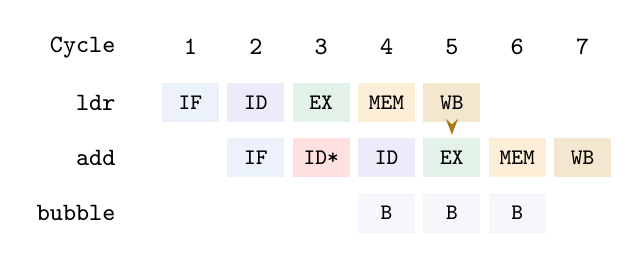
\begin{tikzpicture}[x=0.83cm,y=0.70cm]
\node[anchor=east,font=\small\ttfamily\bfseries] at (0,0) {Cycle};
\node[font=\small\ttfamily] at (1,0) {1};
\node[font=\small\ttfamily] at (2,0) {2};
\node[font=\small\ttfamily] at (3,0) {3};
\node[font=\small\ttfamily] at (4,0) {4};
\node[font=\small\ttfamily] at (5,0) {5};
\node[font=\small\ttfamily] at (6,0) {6};
\node[font=\small\ttfamily] at (7,0) {7};
\node[anchor=east,font=\small\ttfamily,align=right] at (0,-1) {\code{ldr}};
\node[tcell,fill=lightblue] (r1c1) at (1,-1) {IF};
\node[tcell,fill=softpurple] (r1c2) at (2,-1) {ID};
\node[tcell,fill=softgreen] (r1c3) at (3,-1) {EX};
\node[tcell,fill=softorange] (r1c4) at (4,-1) {MEM};
\node[tcell,fill=gold!22] (r1c5) at (5,-1) {WB};
\node[anchor=east,font=\small\ttfamily,align=right] at (0,-2) {\code{add}};
\node[tcell,fill=lightblue] (r2c2) at (2,-2) {IF};
\node[tcell,fill=red!12] (r2c3) at (3,-2) {ID*};
\node[tcell,fill=softpurple] (r2c4) at (4,-2) {ID};
\node[tcell,fill=softgreen] (r2c5) at (5,-2) {EX};
\node[tcell,fill=softorange] (r2c6) at (6,-2) {MEM};
\node[tcell,fill=gold!22] (r2c7) at (7,-2) {WB};
\node[anchor=east,font=\small\ttfamily,align=right] at (0,-3) {bubble};
\node[tcell,fill=softgray] (r3c4) at (4,-3) {B};
\node[tcell,fill=softgray] (r3c5) at (5,-3) {B};
\node[tcell,fill=softgray] (r3c6) at (6,-3) {B};
\draw[bypass] (r1c5.south) -- (r2c5.north);

\end{tikzpicture}\end{center}
\begin{itemize}\setlength{\itemsep}{5pt}
  \item The load produces data at the end of cycle 4. The consumer cannot use it at the start of EX in that same cycle.
  \item Hold the consumer for one cycle, then forward from MEM/WB to EX in cycle 5.
  \item \code{B} = an inactive slot, with no register or memory write.
\end{itemize}

\end{frame}

\begin{frame}{Stall Control and Instruction Scheduling}

\begin{columns}[T,onlytextwidth]
\column{.48\textwidth}
\begin{block}{Hardware Response to Load-Use}
\begin{enumerate}\setlength{\itemsep}{6pt}
\item Hold the PC and IF/ID register.
\item Insert an invalid slot into ID/EX.
\item Let the older load advance normally.
\end{enumerate}
\end{block}
\column{.48\textwidth}
\begin{block}{Independent work fills the gap}
\ttfamily\small
\begin{tabular}{@{}l@{}}
ldr x7, [x5] \\
add x10, x11, x12 \\
add x8, x7, x9
\end{tabular}
\end{block}

\end{columns}
\vspace{.18cm}

\begin{itemize}\setlength{\itemsep}{6pt}
  \item In the reordered sequence, the load reaches MEM in cycle 4 and the dependent \code{add} reaches EX in cycle 5. Forwarding supplies the value without a stall.
  \item Reordering must preserve all register and memory dependencies and other observable effects.
  \item Our model obtains store data in EX, with no special late MEM bypass. A load immediately followed by a store of that loaded value therefore also needs one stall.
\end{itemize}

\end{frame}

\sectiondivider{PART 4}{Control Flow and Pipeline Performance}

\begin{frame}{A Taken Branch Flushes Younger Instructions}

\small\key{Assume:} predict sequential fetch; resolve \code{cbz} in EX; the tested value is zero.
\begin{center}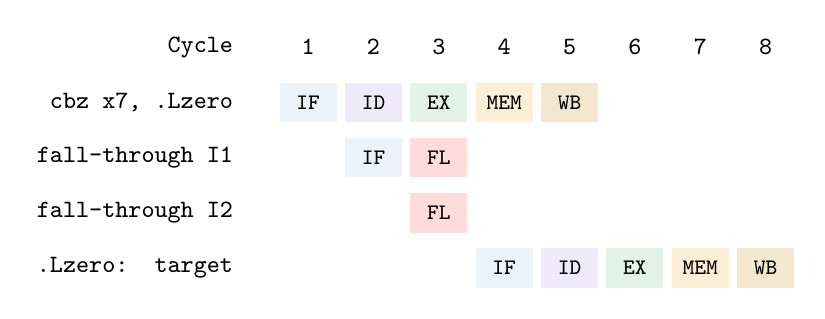
\begin{tikzpicture}[x=0.83cm,y=0.70cm]
\node[anchor=east,font=\small\ttfamily\bfseries] at (0,0) {Cycle};
\node[font=\small\ttfamily] at (1,0) {1};
\node[font=\small\ttfamily] at (2,0) {2};
\node[font=\small\ttfamily] at (3,0) {3};
\node[font=\small\ttfamily] at (4,0) {4};
\node[font=\small\ttfamily] at (5,0) {5};
\node[font=\small\ttfamily] at (6,0) {6};
\node[font=\small\ttfamily] at (7,0) {7};
\node[font=\small\ttfamily] at (8,0) {8};
\node[anchor=east,font=\small\ttfamily,align=right] at (0,-1) {\code{cbz x7, .Lzero}};
\node[tcell,fill=lightblue] (r1c1) at (1,-1) {IF};
\node[tcell,fill=softpurple] (r1c2) at (2,-1) {ID};
\node[tcell,fill=softgreen] (r1c3) at (3,-1) {EX};
\node[tcell,fill=softorange] (r1c4) at (4,-1) {MEM};
\node[tcell,fill=gold!22] (r1c5) at (5,-1) {WB};
\node[anchor=east,font=\small\ttfamily,align=right] at (0,-2) {fall-through I1};
\node[tcell,fill=lightblue] (r2c2) at (2,-2) {IF};
\node[tcell,fill=red!14] (r2c3) at (3,-2) {FL};
\node[anchor=east,font=\small\ttfamily,align=right] at (0,-3) {fall-through I2};
\node[tcell,fill=red!14] (r3c3) at (3,-3) {FL};
\node[anchor=east,font=\small\ttfamily,align=right] at (0,-4) {\code{.Lzero:} target};
\node[tcell,fill=lightblue] (r4c4) at (4,-4) {IF};
\node[tcell,fill=softpurple] (r4c5) at (5,-4) {ID};
\node[tcell,fill=softgreen] (r4c6) at (6,-4) {EX};
\node[tcell,fill=softorange] (r4c7) at (7,-4) {MEM};
\node[tcell,fill=gold!22] (r4c8) at (8,-4) {WB};


\end{tikzpicture}\end{center}
\begin{itemize}\setlength{\itemsep}{5pt}
  \item At the end of cycle 3, redirect the PC and invalidate the younger instruction in ID and the instruction fetched in IF.
  \item Target fetch begins in cycle 4. Two instruction slots are lost under these assumptions.
  \item \code{FL} marks discarded work. Flushes must prevent wrong-path register and memory writes.
\end{itemize}
\note{Control-hazard model: predict not taken, EX resolution. Penalty depends on the implementation.}
\end{frame}

\begin{frame}{AArch64 Branch Operands and Condition Flags}

\begin{columns}[T,onlytextwidth]
\column{.48\textwidth}
\begin{block}{Test a general-purpose register}
\ttfamily\small
\begin{tabular}{@{}l@{}}
cbz  x7, .Lzero \\
cbnz x7, .Lnonzero
\end{tabular}
\end{block}

\begin{itemize}\setlength{\itemsep}{6pt}
  \item Test the value of \code{x7} directly.
  \item Do not read or update NZCV.
  \item The test operand may need forwarding or a load-use stall.
\end{itemize}

\column{.48\textwidth}
\begin{block}{Test condition flags}
\ttfamily\small
\begin{tabular}{@{}l@{}}
cmp  x7, x8 \\
b.eq .Lequal
\end{tabular}
\end{block}

\begin{itemize}\setlength{\itemsep}{6pt}
  \item \code{cmp} updates NZCV; \code{b.eq} tests Z.
  \item \code{cmp} is an alias of \code{subs} with a zero-register destination.
  \item Extending the datapath for this pair requires flag dependence handling.
\end{itemize}

\end{columns}
\vspace{.18cm}
Use the branch instruction\textquotesingle s saved PC for the target. For \code{cbz}/\code{cbnz}, the signed encoded displacement is multiplied by 4.
\note{Arm A64 ISA Guide: compare-and-branch and condition flags. Arm CMP (immediate) instruction reference: alias of SUBS. Timing diagrams use CBZ/CBNZ; NZCV forwarding is an extension.}

\end{frame}

\begin{frame}{Worked Sequence: Load, Add, Store, and Branch}

\small\key{Assume:} the branch is not taken. Forwarding includes store data and the branch test operand.
\begin{center}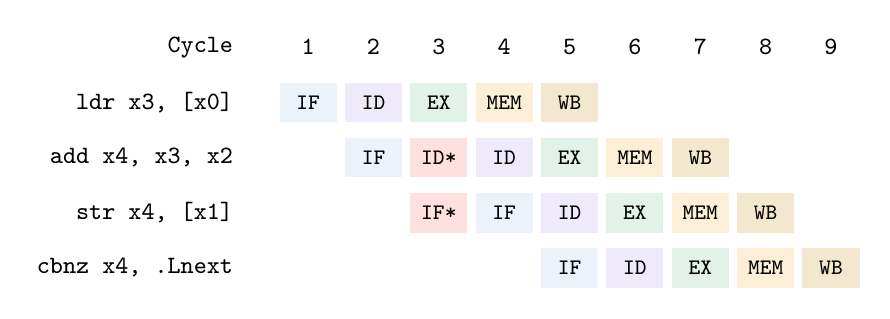
\begin{tikzpicture}[x=0.83cm,y=0.70cm]
\node[anchor=east,font=\small\ttfamily\bfseries] at (0,0) {Cycle};
\node[font=\small\ttfamily] at (1,0) {1};
\node[font=\small\ttfamily] at (2,0) {2};
\node[font=\small\ttfamily] at (3,0) {3};
\node[font=\small\ttfamily] at (4,0) {4};
\node[font=\small\ttfamily] at (5,0) {5};
\node[font=\small\ttfamily] at (6,0) {6};
\node[font=\small\ttfamily] at (7,0) {7};
\node[font=\small\ttfamily] at (8,0) {8};
\node[font=\small\ttfamily] at (9,0) {9};
\node[anchor=east,font=\small\ttfamily,align=right] at (0,-1) {\code{ldr x3, [x0]}};
\node[tcell,fill=lightblue] (r1c1) at (1,-1) {IF};
\node[tcell,fill=softpurple] (r1c2) at (2,-1) {ID};
\node[tcell,fill=softgreen] (r1c3) at (3,-1) {EX};
\node[tcell,fill=softorange] (r1c4) at (4,-1) {MEM};
\node[tcell,fill=gold!22] (r1c5) at (5,-1) {WB};
\node[anchor=east,font=\small\ttfamily,align=right] at (0,-2) {\code{add x4, x3, x2}};
\node[tcell,fill=lightblue] (r2c2) at (2,-2) {IF};
\node[tcell,fill=red!12] (r2c3) at (3,-2) {ID*};
\node[tcell,fill=softpurple] (r2c4) at (4,-2) {ID};
\node[tcell,fill=softgreen] (r2c5) at (5,-2) {EX};
\node[tcell,fill=softorange] (r2c6) at (6,-2) {MEM};
\node[tcell,fill=gold!22] (r2c7) at (7,-2) {WB};
\node[anchor=east,font=\small\ttfamily,align=right] at (0,-3) {\code{str x4, [x1]}};
\node[tcell,fill=red!12] (r3c3) at (3,-3) {IF*};
\node[tcell,fill=lightblue] (r3c4) at (4,-3) {IF};
\node[tcell,fill=softpurple] (r3c5) at (5,-3) {ID};
\node[tcell,fill=softgreen] (r3c6) at (6,-3) {EX};
\node[tcell,fill=softorange] (r3c7) at (7,-3) {MEM};
\node[tcell,fill=gold!22] (r3c8) at (8,-3) {WB};
\node[anchor=east,font=\small\ttfamily,align=right] at (0,-4) {\code{cbnz x4, .Lnext}};
\node[tcell,fill=lightblue] (r4c5) at (5,-4) {IF};
\node[tcell,fill=softpurple] (r4c6) at (6,-4) {ID};
\node[tcell,fill=softgreen] (r4c7) at (7,-4) {EX};
\node[tcell,fill=softorange] (r4c8) at (8,-4) {MEM};
\node[tcell,fill=gold!22] (r4c9) at (9,-4) {WB};


\end{tikzpicture}\end{center}
\begin{itemize}\setlength{\itemsep}{4pt}
  \item \code{ldr} to \code{add}: one stall, then MEM/WB-to-EX forwarding.
  \item \code{add} to \code{str}: forward \code{x4} from EX/MEM into the store-data path in cycle 6.
  \item \code{add} to \code{cbnz}: forward \code{x4} from MEM/WB into the branch test in cycle 7.
  \item The pipeline drains in $4+4+1=9$ cycles. Store and branch WB slots perform no register write.
\end{itemize}

\end{frame}

\begin{frame}{Counting Lost Cycles and Execution Time}

\begin{block}{Finite Run Under the Stated Model}
$\text{cycles}=N+4+S+2B$\\[.1cm]
$S$: load-use stall cycles. \quad $B$: taken branches predicted not taken.\\[.1cm]
Assume the counted penalties do not overlap and occur before the final drain.
\end{block}
\begin{center}
\small
\renewcommand{\arraystretch}{1.28}
\setlength{\tabcolsep}{5pt}
\rowcolors{2}{softgray}{white}
\begin{tabular}{>{\raggedright\arraybackslash}p{7.3cm}>{\raggedright\arraybackslash}p{5.6cm}}
\toprule
\rowcolor{white}
\textbf{Illustrative run} & \textbf{Calculation} \\
\midrule
100 instructions; 10 load-use stalls; 10 taken branches & $100+4+10+2(10)=134$ cycles. \\
Average CPI & $134/100=1.34$. \\
Pipelined time (nanoseconds, ns) & $134\times220\ \mathrm{ps}=29.48$ ns. \\
Single-cycle baseline and speedup & $82$ ns; speedup $82/29.48\approx2.78$. \\
\bottomrule
\end{tabular}
\end{center}

Hazards reduce the achieved speedup below the ideal long-stream value of 3.73.

\end{frame}

\begin{frame}{What the Simple Model Leaves Out}

\begin{itemize}\setlength{\itemsep}{7pt}
  \item \key{Longer operations:} cache misses and multi-cycle arithmetic can hold a stage for several cycles.
  \item \key{Branch prediction:} real implementations may predict both direction and target. Incorrect predictions discard work.
  \item \key{Register ordering:} this model reads in ID and writes in WB, in program order. Out-of-order designs need additional bookkeeping.
  \item \key{AArch64 register views:} \code{w7} and \code{x7} refer to the same register; a write to \code{w7} clears the upper 32 bits of \code{x7}.
  \item \key{More complex instructions:} pre/post-indexed loads, paired transfers, and flag-setting operations need additional datapath and control support.
\end{itemize}

\end{frame}

\begin{frame}{Topic 9 Summary}

\begin{itemize}\setlength{\itemsep}{6pt}
  \item \key{Pipelining:} overlap instructions to increase throughput. The five stages are IF, ID, EX, MEM, and WB.
  \item \key{Clock and timing:} the slowest stage plus register overhead sets the clock period. An ideal $N$-instruction run takes $N+4$ cycles.
  \item \key{Pipeline state:} retain each instruction\textquotesingle s operands, PC, destination, and control signals across stage boundaries.
  \item \key{Data hazards:} forward available results. In our model, an immediate load-use dependence still needs one stall.
  \item \key{Control hazards:} an EX-resolved taken branch flushes two younger slots under sequential prediction.
  \item \key{Correctness:} a store writes memory rather than a register. Bubbles and flushed instructions enable no architectural writes.
\end{itemize}

\end{frame}

\begin{frame}{Self-Test 1: Principles and Timing}

\begin{enumerate}\setlength{\itemsep}{10pt}
\item Explain the difference between instruction latency and instruction throughput. Which does pipelining primarily improve?
\item Stage logic delays are 200, 100, 200, 200, and 100 ps; pipeline-register overhead is 20 ps. Calculate the pipeline clock period and five-stage instruction latency.
\item Eight independent instructions execute in an initially empty five-stage pipeline. How many cycles are needed through final WB? What is the average CPI?
\item Draw a cycle diagram for three independent AArch64 ALU instructions. Which stages are occupied in cycle 3?
\item Why is a five-stage pipeline a microarchitectural choice rather than a requirement of the AArch64 ISA?
\end{enumerate}

\end{frame}

\begin{frame}{Self-Test 2: Datapath and Data Hazards}

\begin{enumerate}\setlength{\itemsep}{8pt}
\item Trace \code{ldr x7, [x5, \#16]} through all five stages. If \code{x5 = 0x1000}, what address is read? What is the unsigned-offset \code{imm12} field?
\item For \code{str x7, [x5, \#16]}, identify the base register and store-data register. Which stage writes memory, and why is \code{RegWrite = 0}?
\item \code{add x7, x5, x6} supplies \code{x7} to a following \code{sub}. Give the forwarding path and stall count. Repeat with \code{ldr x7, [x5]} as the producer; both consumers need \code{x7} in EX.
\item During a load-use stall, which two state elements are held, where is the bubble inserted, and why must the older load continue?
\item Why must a hazard detector recognize a dependence from a write to \code{w7} to a later read of \code{x7}?
\end{enumerate}

\end{frame}

\begin{frame}{Self-Test 3: Control Flow and Performance}

\begin{enumerate}\setlength{\itemsep}{8pt}
\item A taken \code{cbz} resolves in EX in cycle 3 under sequential prediction. Which younger slots are flushed, and in which cycle can target fetch begin?
\item How do the operands of \code{cbz x7, .Lzero} differ from those of \code{cmp x7, x8; b.eq .Lequal}? Which sequence depends on NZCV?
\item For \code{ldr x3, [x0]; add x4, x3, x2; str x4, [x1]}, draw the timing diagram with forwarding. Identify the stall and the path supplying store data.
\item A 100-instruction run has 8 load-use stalls and 6 taken branches predicted not taken. Assume isolated penalties and full drain. Calculate cycles, CPI, and execution time with a 220 ps clock.
\item Why must flushing a wrong-path \code{str} disable its memory write? Would clearing only its register-write control be sufficient?
\end{enumerate}

\end{frame}

% Sources checked while authoring (instruction semantics; model-specific timing is explicitly stated):
% Arm, A64 ISA and Compilers: https://developer.arm.com/community/arm-community-blogs/b/architectures-and-processors-blog/posts/the-a64-isa-and-compilers
% Arm, A64 ISA Guide: https://documentation-service.arm.com/static/68de36a2587fd957f5efc967
% Arm, LDR (immediate): https://support.arm.com/documentation/111181/latest/Base-Instructions/LDR--immediate---Load-register--immediate--
% Arm, CMP (immediate): https://developer.arm.com/documentation/ddi0602/2023-03/Base-Instructions/CMP--immediate---Compare--immediate---an-alias-of-SUBS--immediate--
% Cornell CS3410, pipeline hazards: https://www.cs.cornell.edu/courses/cs3410/2013sp/lecture/09-hazards-w-g.pdf
% Berkeley CS61C, data/control hazards: https://notes.cs61c.org/content/pipeline-hazards/data-hazards/
% https://notes.cs61c.org/content/pipeline-hazards/control-hazards/

\end{document}